\documentclass[12pt]{article}
\usepackage[margin=1in]{geometry}
\usepackage{amsmath, amsthm, amssymb, amsfonts, breqn, graphicx}


\theoremstyle{definition}
\newtheorem{problem}{Problem}
\renewcommand*{\proofname}{Solution}
\newenvironment{custompbm}[1]
  {\renewcommand\theproblem{#1}\problem}
  {\endproblem}
\renewcommand{\theenumi}{\alph{enumi}}


\newcommand{\E}{\text{E}}
\newcommand{\V}{\text{Var}}
\newcommand{\Co}[2]{\text{Cov}\left({#1}, {#2}\right)}
\newcommand{\pdf}{\text{pdf}}
\newcommand{\pmf}{\text{pmf}}
\newcommand{\me}{\mathrm{e}}
\newcommand*\diff{\mathop{}\!\mathrm{d}}
\newcommand{\vect}[1]{\boldsymbol{#1}}
\newcommand{\mx}[1][t]{\mu_X({#1})}
\newcommand{\gx}[2]{\gamma_X({#1}, {#2})}


\title{Homework Assignment 10}
\author{Matthew Tiger}


\begin{document}


\maketitle


\begin{problem}
  Plot the energy bills versus time. What kind of trend appears to exist? What type of seasonal
  variation appears to exist? Is a transformation needed to obtain a series that displays constant
  variation?
\end{problem}

\begin{proof}
  See below for a plot of the bills time series data:
  \vskip 0mm
  \begin{center}
  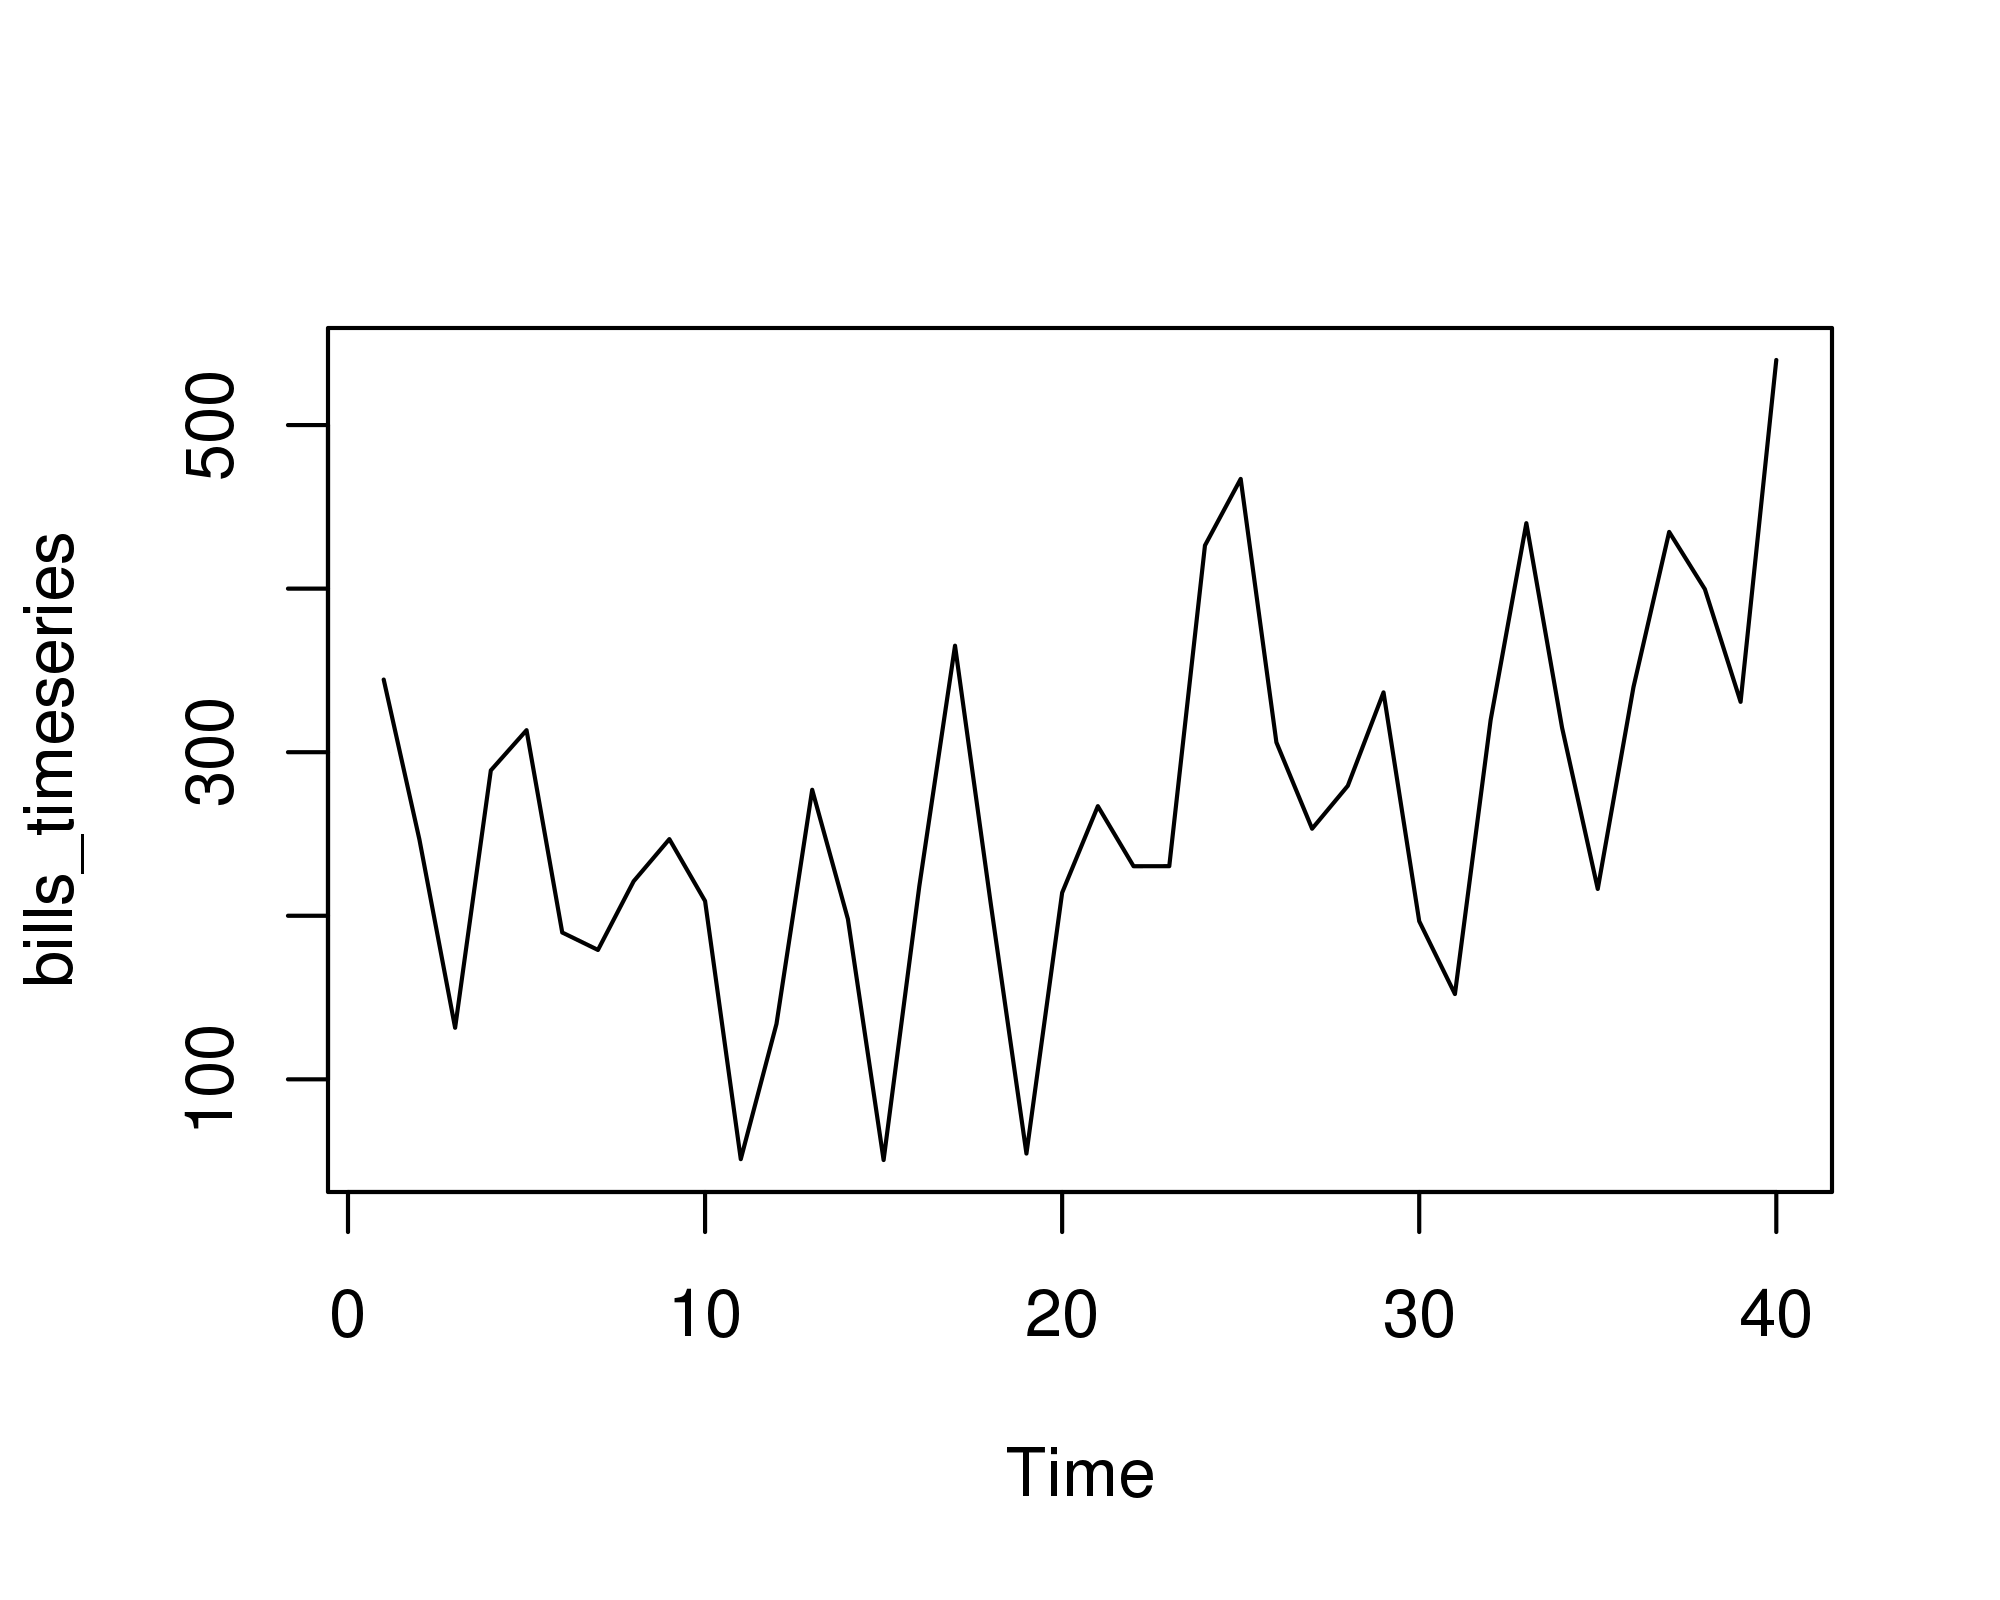
\includegraphics{timeseries}
  \end{center}
  \vskip 10mm

  It is clear from the plot that there is a trend that appears to move upwards
  as time increases and a seasonal variation with period 4
  lags present in the data so a transformation is needed to obtain residuals
  that represent a stationary time series.
\end{proof}


\begin{problem}
  Write algebraically a time series model with trend and seasonal component with definitions
  of the dummy variable.
\end{problem}

\begin{proof}
  As we have both a trend and seasonal component to our data, our model must
  incorporate these facts. Let $\{X_t\}$ represent the observations from our
  original time series. Then $X_t = m_t + s_t + Y_t$ represents our time series model
  where $Y_t$ is a random noise component and $s_t = s_{t+d}$ for some positive integer $d$.

  We can transform this process into a stationary process with repeated applications of the difference
  operator. Assuming the random noise component has zero mean, then the following transformation
  gives us a stationary process with mean $c$:

  $$(1-B)(1-B^4)X_t = c + (1-B)(1-B^4)Y_t$$.
\end{proof}

\end{document}
